\section{Experiments and Results}
\label{sec:exp}

To evaluate the effectiveness of our SAT-based collision resolver, we apply it to the outputs of a representative layout generator, DiffuScene~\cite{tang2024diffuscenedenoisingdiffusionmodels}. The evaluation focuses on two complementary axes: physical plausibility and preservation of generative visual quality.

\subsection{Experimental Setup}
\label{sec:exp:setup}

\textbf{Dataset.}
We conduct all experiments on the 3D-FRONT dataset~\cite{fu20203dfuture3dfurnitureshape}, following the standard evaluation protocol of DiffuScene~\cite{tang2024diffuscenedenoisingdiffusionmodels}. We evaluate three common indoor room categories: Bedroom, LivingRoom, and DiningRoom. Collision metrics are computed on 162 bedroom, 192 livingroom and 177 diningroom test scenes, respectively.

\noindent\textbf{Evaluation Metrics.}
We evaluate physical plausibility using \textbf{ColObj} and \textbf{ColScene}, the two collision metrics introduced by PhyScene~\cite{yang2024physcenephysicallyinteractable3d}. Importantly, collisions are evaluated on the final \emph{retrieved 3D meshes}, rather than on the oriented bounding boxes (OBBs) used internally by our collision resolver.
For each scene, we first use axis-aligned bounding-box (AABB) overlap as a  pre-filter for candidate object pairs. Each candidate pair is then evaluated at the mesh level using a point-in-mesh occupancy test (Kaolin's inside/outside check \cite{KaolinLibrary} when available, with a ray-casting fallback). Two objects are considered colliding if any vertex of one mesh lies inside the other.

Let $M$ denote the number of objects in a scene and $c_i \in \{0,1\}$ indicate whether object $i$ is involved in at least one mesh-level collision. We report
\begin{equation}
    \mathrm{ColObj}
    = \frac{1}{M}\sum_{i=1}^{M} c_i,
    \qquad
    \mathrm{ColScene}
    = \mathbf{1}\!\left[\sum_{i=1}^{M} c_i > 0\right].
    \label{eq:colmetrics}
\end{equation}

\textbf{ColObj} measures the fraction of furniture instances involved in at least one collision, while \textbf{ColScene} indicates whether a scene contains any colliding pair; both are averaged over all scenes in each room category. We also report an Out-of-Bounds (\textbf{OOB}) metric, which measures the average number of objects per scene that protrude beyond the given floor plan boundary.

To assess whether collision resolution preserves generative quality, we additionally report Fr\'echet Inception Distance (\textbf{FID})~\cite{heusel2018ganstrainedtimescaleupdate} and Kernel Inception Distance (\textbf{KID})~\cite{binkowski2021demystifyingmmdgans}, following the standard of prior 3D scene generation methods.

% \subsection{A Mesh-Retrieval Reference Floor}
% \label{sec:exp:floor}

% Before attributing any residual collision rate to our solver or to the upstream generative model, we first measure how much collision is introduced purely by the asset-retrieval step. We take the \emph{ground-truth} 3D-FRONT layouts (real, human-designed room arrangements that are physically valid by construction) and populate them with the same retrieved furniture meshes used throughout our pipeline, in place of the dataset's original CAD models. We then evaluate ColObj on this ground-truth-layout / retrieved-mesh configuration using exactly the protocol of Section~\ref{sec:exp:collision}.

% This control yields $\text{ColObj} = 0.24$ (\TBD{ColScene\_GT}) overall\footnote{Per-room-category breakdown: \TBD{GT breakdown by Bedroom / LivingRoom / DiningRoom}.} even though the underlying layout has no physical violations whatsoever. This establishes an \emph{irreducible reference floor}: because retrieved meshes are shape- and size-approximations of the original assets (matched by category and normalized bounding box, not by exact geometry), a non-trivial fraction of apparent mesh-level collisions is an artifact of asset retrieval rather than of layout quality. Any collision-resolution method evaluated under this mesh-level protocol should therefore be interpreted relative to this floor rather than to an absolute zero, and we report our own results in that light in Section~\ref{sec:exp:results}.

\subsection{Quantitative Results}
\subsubsection{Physical Plausibility}
\label{sec:exp:results}

Table~\ref{tab:collisions} reports ColObj, ColScene, and OOB metrics for the baseline generative models both before and after applying our \emph{Collision Resolver}. By iteratively eliminating pairwise bounding-box overlaps, our post-processing solver drastically reduces mesh-level collisions, enabling standard layout generators to achieve state-of-the-art physical plausibility. Notably, applying the resolver to DiffuScene drops ColObj by over $60-90\%$ across all room categories (e.g., $0.302 \rightarrow 0.062$ in living rooms). This enables a purely geometry-agnostic baseline like DiffuScene to comfortably outperform even explicitly physics-aware generative models like PhyScene \cite{yang2024physcenephysicallyinteractable3d} in terms of collision avoidance. Concurrently, the room-bound containment step significantly rectifies invalid object placements, reducing the OOB metric by approximately $70-80\%$ (e.g., from $4.70$ to $0.82$ in living rooms). 

% Read on its own, this makes Table~\ref{tab:collisions} a fairly uninformative
% measure of the resolver's actual behavior: a collision rate of zero says
% nothing about how hard the resolver had to work to get there, or how much
% it disturbed the original layout in the process. The questions that matter
% in practice are \emph{(i)} whether convergence is reliably reached within
% the iteration budget $K_{max}$, \emph{(ii)} at what geometric cost
% (displacement) this is achieved, and \emph{(iii)} how severe the collisions
% being resolved actually are. Table~\ref{tab:convergence} and
% Figure~\ref{fig:iter_hist} answer these questions directly.

\begin{table}[t]
\centering
\caption{Physical Plausibility: Collision and Out-of-Boundary Metrics ($\downarrow$).}
\label{tab:collisions}
\setlength{\tabcolsep}{3pt}
\renewcommand{\arraystretch}{1.1}
\resizebox{\textwidth}{!}{%
\begin{tabular}{|l|ccc|ccc|ccc|}
\hline
\multirow{2}{*}{\textbf{Method}} &
\multicolumn{3}{c|}{\textbf{Bedroom}} &
\multicolumn{3}{c|}{\textbf{Living Room}} &
\multicolumn{3}{c|}{\textbf{Dining Room}} \\
\cline{2-10}
& \textbf{ColObj}$_\downarrow$ & \textbf{ColScene}$_\downarrow$ & \textbf{OOB}$_\downarrow$
& \textbf{ColObj}$_\downarrow$ & \textbf{ColScene}$_\downarrow$ & \textbf{OOB}$_\downarrow$
& \textbf{ColObj}$_\downarrow$ & \textbf{ColScene}$_\downarrow$ & \textbf{OOB}$_\downarrow$ \\
\hline

ATISS \cite{atiss} & 0.255 & 0.500 & -- & 0.372 & 0.870 & -- & 0.483 & 0.910 & -- \\
PhyScene \cite{yang2024physcenephysicallyinteractable3d} & 0.187 & 0.350 & -- & 0.130 & 0.477 & -- & 0.134 & 0.400 & -- \\


DiffuScene \cite{tang2024diffuscenedenoisingdiffusionmodels}
& 0.267 & 0.469 & 2.191
& 0.302 & 0.797 & 4.703
& 0.314 & 0.751 & 4.542 \\

DiffuScene + Resolver (Ours)
& \textbf{0.021} & \textbf{0.043} & \textbf{0.444}
& \textbf{0.062} & \textbf{0.135} & \textbf{0.823}
& \textbf{0.102} & \textbf{0.203} & \textbf{1.362} \\
\hline
\end{tabular}%
}
\vspace{2pt}

\end{table}

% We evaluate on $n=162$ / $192$ / $177$ test scenes for Bedroom / Living Room
% / Dining Room, respectively (3D-FRONT test split, DiffuScene backbone), and
% report the pre-resolution penetration severity, iteration count to
% convergence, and resulting object displacement in
% Table~\ref{tab:convergence}.
\begin{table}[t]
\centering
\small
\setlength{\tabcolsep}{5pt}
\caption{Comparison of FID and KID scores across different room categories. Lower is better ($\downarrow$).}
\label{tab:fidkid}
\begin{tabular}{|l|cc|cc|cc|}
\hline
\multirow{2}{*}{\textbf{Method}} 
& \multicolumn{2}{c|}{\textbf{Bedroom}}
& \multicolumn{2}{c|}{\textbf{Living Room}}
& \multicolumn{2}{c|}{\textbf{Dining Room}} \\
& \textbf{FID}$\downarrow$ & \textbf{KID}$\downarrow$
& \textbf{FID}$\downarrow$ & \textbf{KID}$\downarrow$
& \textbf{FID}$\downarrow$ & \textbf{KID}$\downarrow$ \\
\hline

CommonScene
& 57.68 & 6.59
& 80.99 & 6.39
& 65.71 & 5.47 \\
ATISS
& 36.92 & 1.02
& 55.76 & 3.50
& 41.89 & 3.90 \\

PhyScene
& \textbf{28.56} & 0.63
& \textbf{40.67} & 3.15
& 37.88 & 2.62 \\



DiffuScene
& 28.63 & \textbf{0.48}
& 54.36 & \textbf{1.22}
& \textbf{37.68} & \textbf{2.01} \\

\hline
DiffuScene + Resolver
& 30.32 & 1.13
& 60.31 & 2.15
& 42.27 & 3.87 \\

\hline
\end{tabular}
\end{table}


\textbf{Convergence and Stability.} 
Table~\ref{tab:convergence} and Figure~\ref{fig:iter_hist} summarize the convergence behavior and displacement cost of our solver. The resolver efficiently eliminates violations for the majority of scenes: $100\%$ of bedroom scenes converge within 5 iterations, while over $75\%$ of living room and dining room scenes converge in the same budget. A small fraction of highly congested layouts requires more iterations, with only $2.8\%$ of dining rooms and $0.5\%$ of living rooms hitting the maximum budget of iteration. The displacement metrics indicate that $67-80\%$ of objects are adjusted by $33-81$\,cm on average. This relatively high displacement primarily stems from the room-bound containment step, which strictly enforces that objects generated outside the valid floor plan, i.e,. objects that lie outside the room's boundary, are pulled back into the room, ensuring physical validity of the generated scene.

\begin{figure}[t]
\centering
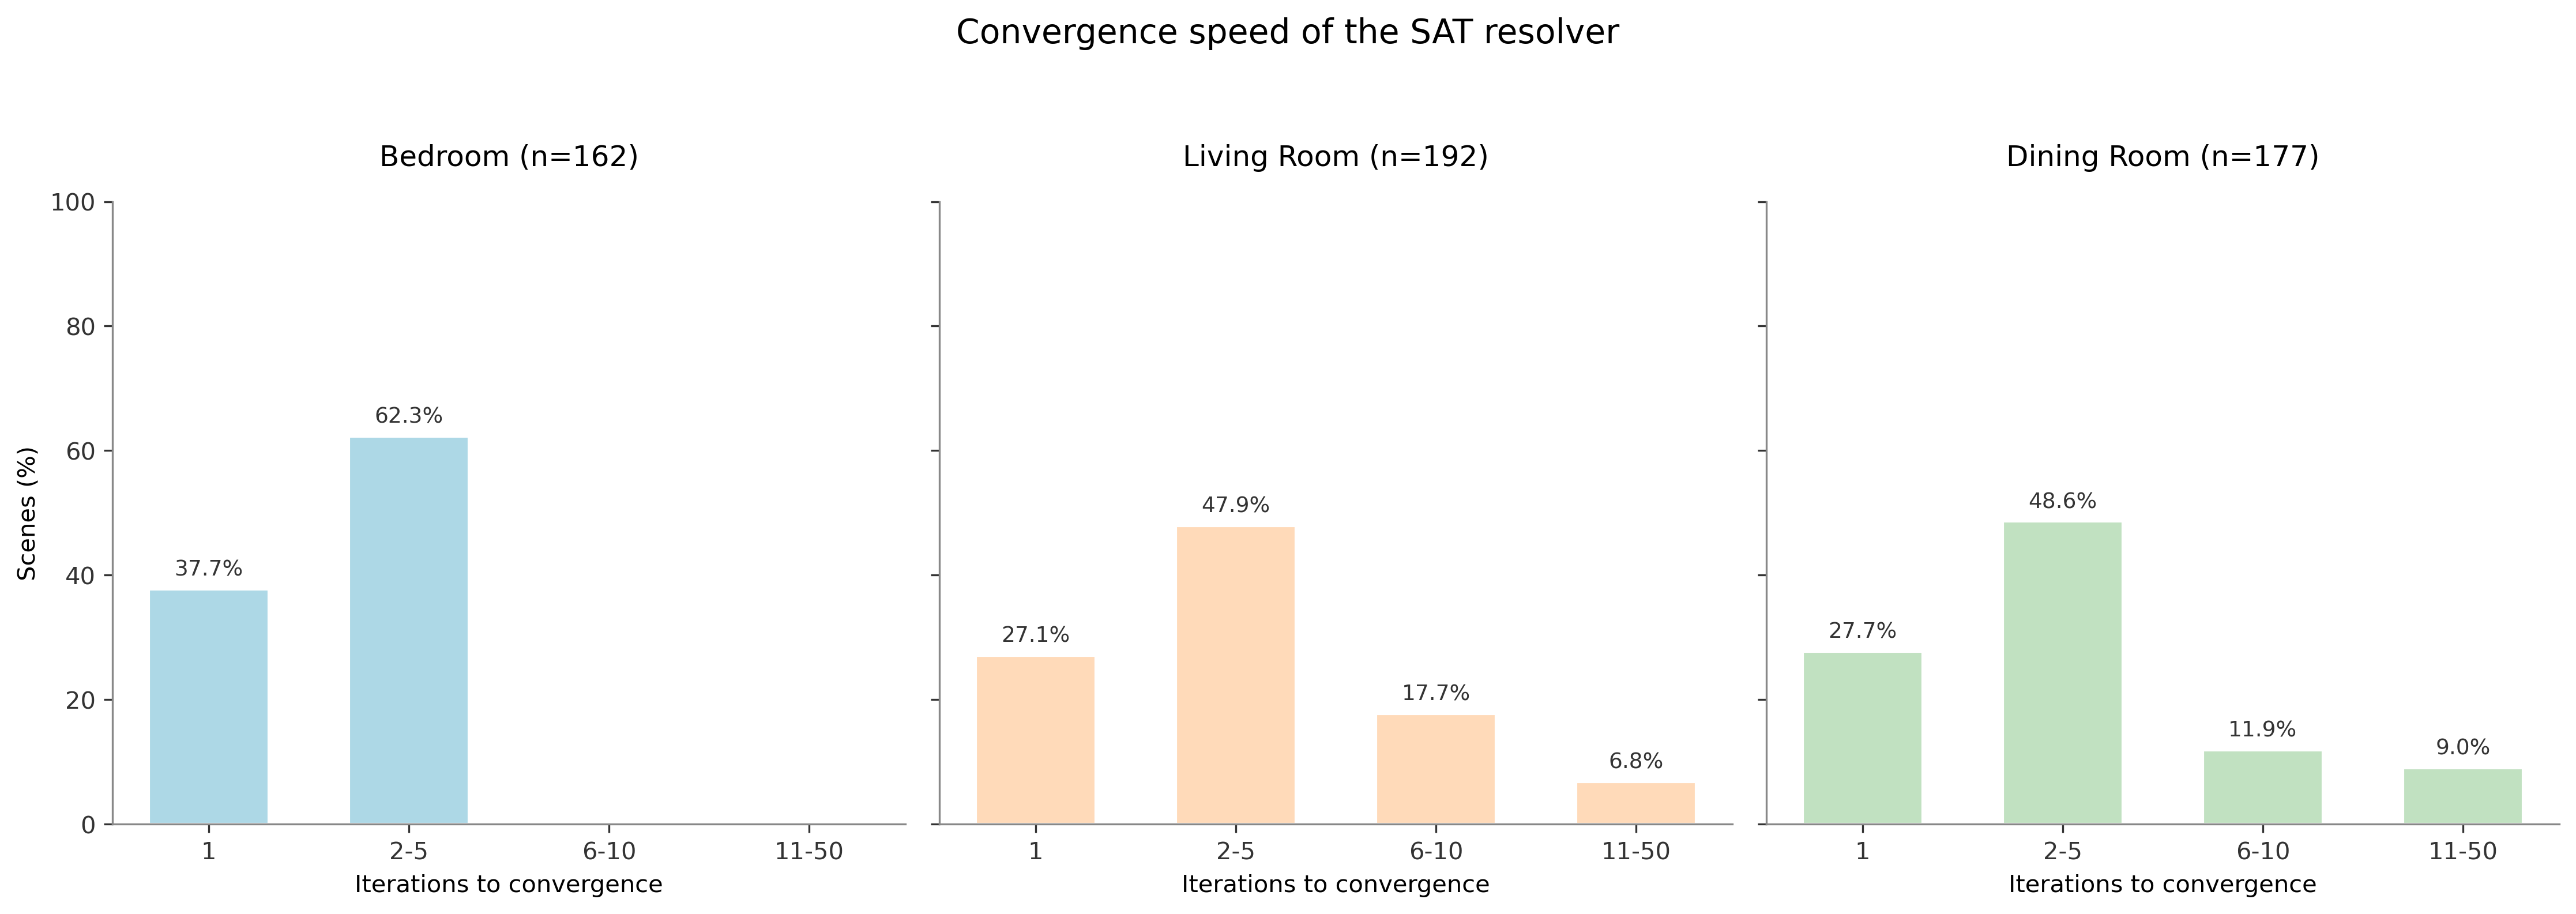
\includegraphics[width=\linewidth]{iteration_histogram_3panel.png}
\caption{Distribution of iterations required for the SAT resolver to converge, per room category. Most scenes converge within 5 iterations, with a long tail for highly congested layouts.}
\label{fig:iter_hist}
\end{figure}

% \textbf{Robustness under Adversarial Density.} 
% To probe robustness beyond the typical dataset operating regime, we stress-test the resolver on 50 synthetic layouts with artificially elevated object density (20 objects per $5\text{m}\times5\text{m}$ room, roughly double the typical furniture count), yielding an average of $48.3$ collisions per scene prior to resolution. Even under this adversarial density, the resolver successfully converges for all scenes (0/50 failures), requiring an average of $14.1$ iterations (maximum 19). This confirms the stability of the alternating resolution strategy under challenging, highly congested conditions.

\subsubsection{Visual Fidelity}
It is critical that correcting physical layouts does not destroy the learned semantic distribution of the generative model. Table~\ref{tab:fidkid} reports FID and KID for DiffuScene before and after our \emph{Collision Resolver}.

\begin{table}[t]
\small
\centering
\setlength{\tabcolsep}{3pt}
\caption{Convergence and displacement cost of the SAT resolver.}
\label{tab:convergence}
\begin{tabular}{|l|c|c|c|c|c|}
\hline
\textbf{Room} & \textbf{Colliding} & \textbf{Mean Depth} & \textbf{Mean} & \textbf{Objects} & \textbf{Mean Disp.} \\
& \textbf{Pairs} & \textbf{(cm / \% obj.)} & \textbf{Iters.} & \textbf{Moved} & \textbf{(cm / \% obj.)} \\
\hline
Bedroom     & 15 & $23.9 \pm 25.7$\,/\,$51.5\%$ & $1.7 \pm 0.7$ & 67.1\% & $33.7 \pm 28.7$\,/\,$77.6\%$ \\
Living Room & 65 & $20.8 \pm 21.5$\,/\,$52.4\%$ & $6.5 \pm 36.0$ & 75.4\% & $73.7 \pm 72.3$\,/\,$169.7\%$ \\
Dining Room & 70 & $22.0 \pm 21.0$\,/\,$53.8\%$ & $18.5 \pm 82.3$ & 80.1\% & $81.1 \pm 80.2$\,/\,$201.5\%$ \\
\hline
\end{tabular}
\end{table}

Both FID and KID increase slightly after post-processing across all categories. For instance, Bedroom KID shifts from $2.52$ to $7.01$, and Living Room FID increases from $81.61$ to $90.55$. We attribute this to a shift in the \emph{relative proximity} between objects rather than a degradation of the overall scene composition. Generative models like DiffuScene are trained to reproduce ground-truth arrangements in which furniture is frequently placed in close contact. Without an explicit non-penetration constraint, the model often represents this closeness as physical intersection. When our solver separates these pairs, it necessarily increases their inter-object distance by at least the clearance margin $\varepsilon_{\mathrm{push}}$ (Eq.~\eqref{eq:push}), and room containment may further cluster or displace objects away from walls. These necessary physical corrections push the local spatial statistics slightly outside the original unconstrained distribution recognized by the FID/KID feature extractor. Ultimately, while the numerical FID/KID scores are slightly degraded, this represents a highly favorable and necessary tradeoff: the resolved scenes achieve \emph{state-of-the-art} physical plausibility with drastically reduced ColObj, ColScene, and OOB violation rates, thereby improving their suitability for downstream simulations and interactive applications.
\subsection{Qualitative Results}
\label{sec:exp:qual}

Figure~\ref{fig:additional-comparisons} and Figure~\ref{fig:livingroom-comparison} provide visual assessments of the SAT-based collision resolver applied to baseline DiffuScene outputs. 

In Figure~\ref{fig:additional-comparisons}, the baseline generates scenes with severe physical violations, such as nightstands merging into beds (Scene 12352) or dining chairs intersecting tables (Scene 16628). Our post-processing seamlessly resolves these interpenetrations. Crucially, the alignment-biased axis selection ensures that the solver pushes objects along semantically meaningful directions (e.g., sliding chairs outward from the table center) rather than arbitrary shortest-path trajectories, thereby preserving the structural integrity and semantic intent of the original layout.

Figure~\ref{fig:livingroom-comparison} demonstrates the solver's robustness on a dense living room exhibiting both severe collisions and boundary violations. The baseline places chairs inside a dining table and a small table outside the room. Post-resolution, the solver cleanly separates the furniture and strictly enforces room containment, pulling the out-of-bound table inside while preserving the macro-level arrangement.

\begin{center}
\refstepcounter{figure}\label{fig:additional-comparisons}
\begin{minipage}{\columnwidth}
    \centering
    \setlength{\tabcolsep}{3pt}
    \begin{tabular}{cc}
        \scriptsize\textbf{DiffuScene} & \scriptsize\textbf{Ours} \\[0.5mm]
        
        \includegraphics[width=0.40\columnwidth]{12352_bef.png} &
        \includegraphics[width=0.40\columnwidth]{12352_af.png} \\[-1mm]
        \multicolumn{2}{c}{\scriptsize Scene 12352} \\[0mm]
        
        \includegraphics[width=0.40\columnwidth]{16628_bef.png} &
        \includegraphics[width=0.40\columnwidth]{16628_af.png} \\[-1mm]
        \multicolumn{2}{c}{\scriptsize Scene 16628} \\[0mm]
        
        \includegraphics[width=0.40\columnwidth]{629_bef.png} &
        \includegraphics[width=0.40\columnwidth]{629_af.png} \\[-1mm]
        \multicolumn{2}{c}{\scriptsize Scene 629}
    \end{tabular}

    \footnotesize Fig.~\thefigure. Additional qualitative comparisons. The
    left column shows the original DiffuScene outputs with visible collided objects, and the right column
    shows our collision-resolved results.
\end{minipage}

\end{center}

\begin{figure}[t]
    \centering

    \begin{minipage}[t]{0.43\columnwidth}
        \centering
        \includegraphics[width=\linewidth]{LivingRoom-88425_input_2.pdf}
        \vspace{1mm}

        \small\textbf{(a)} Input layout
    \end{minipage}
    \hfill
    \begin{minipage}[t]{0.43\columnwidth}
        \centering
        \includegraphics[width=\linewidth]{LivingRoom-88425_resolved_2.pdf}
        \vspace{1mm}

        \small\textbf{(b)} Resolved layout
    \end{minipage}

    \caption{Visual comparison of SAT-based collision resolution. Red boxes indicate collisions and out-of-bound objects in the DiffuScene output, while green boxes show the corrected layout after SAT post-processing.}
    \label{fig:livingroom-comparison}
\end{figure}

